% slides.tex
\documentclass[aspectratio=169,20pt]{beamer}
\usepackage{listings}
\usepackage[utf8]{inputenc}
\usepackage{cancel}
\usepackage{color}
\usepackage{graphicx}
\usepackage{pdfpages}
\usepackage{amsmath}
\usepackage{xcolor}

\usetheme{default}
\usecolortheme{dove}
\useoutertheme{default}

% Remove navigation symbols
\setbeamertemplate{navigation symbols}{}

% Slightly smaller title
\setbeamerfont{frametitle}{size=\large}
\setbeamerfont{verb}{size=\small}

% Font
\renewcommand{\ttdefault}{pcr}

% lst settings
\lstset{
    basicstyle=\ttfamily\footnotesize,
    gobble=4,
    keywordstyle=\ttfamily\bfseries,
    showstringspaces=false
}

\newcommand{\vspaced}{
    \vspace{5mm}
}

\newcommand{\fullimageframe}[1]{
    {
        \usebackgroundtemplate{
            \includegraphics[height=\paperheight,width=\paperwidth]{#1}}
        \setbeamertemplate{navigation symbols}{}
        \begin{frame}[plain]
        \end{frame}
    }
}

\newcommand{\imageframe}[1]{
    {
        \begin{frame}[plain]
        \begin{center}
        \includegraphics[width=\textwidth]{#1}
        \end{center}
        \end{frame}
    }
}

\newcommand{\chapterslide}[1]{
    {
        \begin{frame}[plain]
        \begin{center}
        \large{#1}
        \end{center}
        \end{frame}
    }
}

\newcommand{\blackslide}[1]{
    {
        \setbeamercolor{background canvas}{bg=black}
        \chapterslide{\color[rgb]{1,1,1}{#1}}
    }
}

\newcommand{\code}[1]{
    \texttt{\small{#1}}
}

\definecolor{asparagus}{rgb}{0.53, 0.66, 0.42}
\definecolor{bittersweet}{rgb}{1.0, 0.44, 0.37}

\begin{document}

\title{Composable Infrastructure through FP}
\subtitle{Comcast Labs Connect FP conference}
\author{Jasper Van der Jeugt}
\date{March 9, 2018}

\begin{frame}[plain]
    \titlepage
\end{frame}

\begin{frame}{About me}
    % - First learned about Haskell at university from a friend
    % - Pretty deep into Ruby and Lua at that time
    % - So thanks for redeeming me
    \begin{itemize}
    \item Discovered FP at Uni, haven't looked back
    \item Contributed to and authored open source projects
    \item Worked with Haskell for some companies
    \item Currently at Fugue
    \end{itemize}
\end{frame}

\begin{frame}{Fugue}
    % - I think the idea of Fugue fairly simple
    % - Express everything beautifuly, concisely in a composable way
    % - Fugue makes it so
    % - Eventually taken very liberally
    %
    % - The language in which you specify infrastructure but also rules is
    %   called Ludwig
    % - Only a small part of Fugue uses Haskell but we have fully adopted the
    %   functional mindset
    % - Immutable infrastructure encouraged
    \emph{Fugue} is a cloud orchestration platform that offers a variety of
    services \\
    \vspaced
    The single source of truth for Fugue is defined in a functional,
    statically typed language called \emph{Ludwig} \\
\end{frame}

\begin{frame}{FP and Infrastructure}
    % - This is case study talk, an experience report
    % - What are our reasons for using FP
    % - What language features are important to us?
    % - How do we teach functional programming?
    % - Can't say "Go read category book"
    This talk is about our experience with applying FP to this domain that
    encompasses a few different topics such as compliance, DevOps, immutability
    infrastructure\ldots
\end{frame}

\begin{frame}{FP and Infrastructure}
    % - This is a technical conference so I don't want to convert anyone today
    % - But if you're using CFN, why not generate it from Haskell
    % - Or lisp, but then you'd run into trouble LOL
    % - Make you think about configuration management, especially as it relates
    %   to cloud since there's a lot of it
    % - If your config is less than 100 lines you probably don't care
    I'm using Ludwig as a case study but most things in this talk generalize to
    other languages which share the traits we all love such as Hindley–Milner
    type inference, referential transparency, immutability, row types\ldots
\end{frame}

% - Don't want to get philosophical dont worry
% - Also dont want to get too theoretic
% - But it's "configuration management" and nobody seems to have a clue what
%   management entails so it would be good if we could talk about at least one
%   of these two words
\chapterslide{What's in a configuration?}

\begin{frame}[fragile]{Keeping it Simple\textsuperscript{\tiny{TM}} with JSON}
    % - Simple example to start with
    % - Records
    % - Some different values of different types
    % - Lists as well
    % - There's also INI config file format (or any of the thousand)
    % - What's the advantage of JSON?  You can put JSON in JSON!!!
    \begin{lstlisting}
    {
      "loadBalancer": {
        "port": 80,
        "name": "my-elb",
        ...
      }
    }
    \end{lstlisting}
\end{frame}

\begin{frame}{Keeping it Simple\textsuperscript{\tiny{TM}} with JSON}
    % - Immutable means that I'm not modify to change it 10 lines down
    % - That you don't need to browse through it to figure out state
    % - Things have types I suppose
    % - JSON schemas are a thing and are actually not that bad
    % - Tooling is ATROCIOUS
    %
    % - Making the step to typed will give us many, many advantages...
    Common (sane) configuration use cases of JSON are already: \\
    \vspaced
    \begin{itemize}
    \item Immutable
    \item \emph{Mostly} typed
    \end{itemize}
    \vspaced
\end{frame}

\begin{frame}[fragile]{Types}
    % - I've now changed this JSON to Ludwig
    % - The quotes dissapeared
    % - This makes it easy to learn: its just JSON
    % - if you're not doing anything advanced its just JSON with good errors
    \begin{lstlisting}
    {
      loadBalancer: {
        port: 80,
        name: "my-elb",
        ...
      }
    }
    \end{lstlisting}
\end{frame}

\begin{frame}[fragile]{Types}
    % - We can actually look at the type now
    % - Record typing, even typescript has (some form of it)
    % - There's a few different approaches and I'll get into that a bit later
    % - Simple to read, intuitive to understand, simple to infer(?)
    \begin{lstlisting}
    {
      loadBalancer: {
        port: Int,
        name: String,
        ...
      }
    }
    \end{lstlisting}
\end{frame}

\begin{frame}{Types}
    % - I'm the author of NGINX
    % - I provide a type definition of the config I expect
    % - People can browse it, check it
    % - Prevents a class of weird runtime errors
    % - Always typed, port == Int
    % - Some things are just... weirdly typed, unsound, no principal times
    % - Show multiple errors VS show one error VS runtime BOOM
    % - An example can never be exhaustive
    % - Dependent types PLEASE
    What happens if we write a type definition for our JSON configuration? \\
    \vspaced
    \begin{itemize}
    \item Generate \emph{useful} error messages
    \item Show multiple errors at once!
    \item Generate documentation
    \end{itemize}
\end{frame}

\begin{frame}{Types}
    % - I firmly believe
    % - Outweigh the downsides
    % - Slower on startup only
    % - Client request to your webserver should still be JSON
    % - More bugs, bigger to install, harder to embed, more to learn
    There's always downsides\ldots
    \vspaced
    \begin{itemize}
    \item No more \texttt{[null, 4, "Four"]}
    \item Obviously \emph{significantly} slower
    \item Additional components means more complexity
    \end{itemize}
\end{frame}

\begin{frame}{Types}
    % - My favorite paper (or its in my top three)
    % - Present this at local Zurich papers we love
    % - Offers more power than what we need
    % - At the same time being simpler than what we want
    %
    % - Error messages are not great though
    % - Need some special cases
    % - But yeah I think error messages are hard, not enough formalization
    %   around here
    There are many ways to infer types \\
    For configuration management, row types are \emph{really} important \\
    \vspaced
    \emph{Extensible records with scoped labels} \\
    by Daan Leijen - 2005
\end{frame}

% - Is this all needed?
% - Anonymous functions
% - Let bindings etc
% - Hell yeah I want that
\chapterslide{Why such a ``complex'' system?}

\begin{frame}[fragile]{Configuration is Hard}
    % - NGINX config
    % - I thought you said you dont allow nesting
    % - Well there is some nesting, sometimes allowed, sometimes disallowed
    %   which is even weirder
    % - Oh I guess `index.html` is a list like thing?  I hope it's clearly not a
    %   filename with spaces in there
    % - But alright alright alright I'll confess this is pretty simple
    \begin{lstlisting}
    server {
      listen      80;
      server_name localhost;
      location / {
        root   html;
        index  index.html index.htm;
      }
    }
    \end{lstlisting}
\end{frame}

\blackslide{Two weeks later\ldots}

\begin{frame}[fragile]{Configuration is Hard}
    % - Maybe it's a nightmare and you wake up
    % - But you must've gotten these nightmares somewhere
    % - I suppose it's a programming language heavily inspired by bash
    % - When I think a language needs more power I look at Lisp, Haksell but
    %   even sometimes C, Python (which has some great ideas)
    \begin{lstlisting}
    if ( $remote_addr != 10.11.12.13 ) {
      set $check G;
    }
    if ( -f $document_root/maintenance.html){
      set $check "${check}O";
    }
    if ( $check = GO ) {
      return 503;
    }
    \end{lstlisting}
\end{frame}

\begin{frame}{}
    \begin{center}
    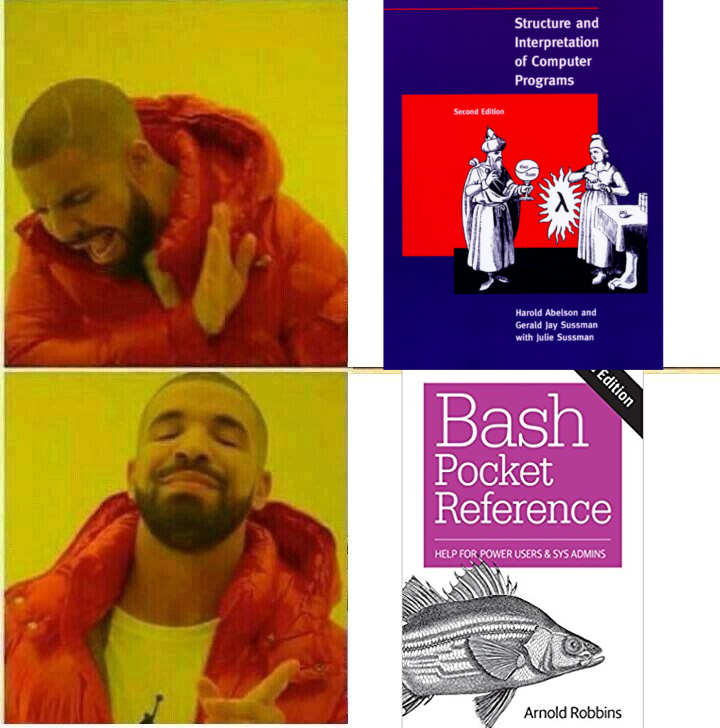
\includegraphics[height=0.9\paperheight]{images/sicp-vs-bash.png}
    \end{center}
\end{frame}

\begin{frame}[fragile]{Keeping it Simple\textsuperscript{\tiny{TM}} with YAML}
    % - So right I'm not gonna invent my own flat format
    % - Let's use structured YAML
    % - This is simple and nice, plus types
    % - Oh look it's immutable (and Ansible got that right)
    % - Actually not really immutable, but at least Idempotent
    % - The language doesn't actively prevent this
    \begin{lstlisting}
    - name: add my user
      user:
        name: "jasper"
        state: present
        groups: "wheel"
    \end{lstlisting}
\end{frame}

\blackslide{Ten minutes later...}

\begin{frame}[fragile]{Keeping it ``Simple''\textsuperscript{\tiny{TM}} with YAML}
    % - The type depends on `with_items` being present
    % - I don't think dependent types can capture that elegantly and even if
    %   they can I wouldn't want to implement that
    % - Is this lexically scoped?  Maybe
    % - Is this always called item?
    % - What if I want to call it something else or differently?
    % - Or a nested loop?  I HAVE SO MANY QUESTIONS
    \begin{lstlisting}
    - name: add several users
      user:
        name: "{{ item }}"
        state: present
        groups: "wheel"
      with_items:
         - testuser1
         - testuser2
    \end{lstlisting}
\end{frame}

\begin{frame}{Configuration is Hard}
    % - I hope everyone is familiar with this
    % - Scripting language
    % - If you don't look existing research
    % - Most famous example: VIM
    % - I am a VIM user myself but I can't really configure it too well because
    %   I've never bothered learning VIMSCRIPT
    % - But I envy Emacs users when it comes to their extensible configuration
    %   format
    %
    % - So I would like to propose an analogue
    % - Any sufficiently advanced configuration format contains an ad-hoc,
    %   informally specified, bug-ridden slow implementation of for loops and if
    %
    % - This is not a great situation to be in
    \textbf{Greenspun's tenth rule of programming:} \\
    \vspaced
    \emph{Any sufficiently complicated C or Fortran program contains an ad-hoc,
    informally-specified, bug-ridden, slow implementation of half of Common
    Lisp.}
\end{frame}

% - Explain how it looks
% - Relate to assembly
%
% - Examples: HTML, (Assembly+JavaScript), Bitmaps, Programming languages
\fullimageframe{images/cartesian-01.pdf}
\fullimageframe{images/cartesian-02.pdf}

\begin{frame}[fragile]{Control structures}
    % - We can only do this BECAUSE we quoted my-elb and because we didn't quote
    %   port
    % - It can go in two ways: we reserve space for it, or we add it from the
    %   beginning
    % - We're not gonna need it, and build on the assumption that you don't need
    %   it
    %
    % - I'm using sum types here.  That's pretty good for modelling Prod/Dev
    % - Because you could add a param, but I digress
    % - It's easy to read
    %
    % - Not spaghetti!  We can't modify anything!
    Embrace control structures rather than half-heartedly bolting them
    on! \\
    \vspaced
    \begin{lstlisting}
    loadBalancer: {
      port: if env == Prod then 80 else 8080,
      name: "my-elb",
      ...
    }
    \end{lstlisting}
\end{frame}

\begin{frame}[fragile]{Control structures}
    % - What else is nice about Haskell?
    % - We don't have for loops
    % - But we have LIST COMPREHENSIONS
    % - Surprisingly people are familiar with this (THANKS PYTHON)
    % - Python's list comprehensions aren't nested but the idea is easy
    \begin{lstlisting}
    loadBalancers: [
      {
        port: port
        name: name
        ...
      } for (port, name) in elbList
    ]
    \end{lstlisting}
\end{frame}

\begin{frame}{Control structures}
    % - Yes we have list comprehensions so we can repeat things
    % - But not accross different files
    % - Not very readable
    Even \emph{with} powerful control structures we still end up copying
    pasting the same lines of codes from stackoverflow\ldots
\end{frame}

\begin{frame}
    What we really want is some form of stored \emph{examples}, \emph{templates}
    or \emph{recipes} that we can customize to our needs, but they should
    \emph{compose} well and not interfere with each other\ldots
\end{frame}

% - There are many different kinds of module systems
% - Doesn't matter too much for the purpose of this talk
\chapterslide{Functions functions functions! \\
\small{(And a simple sane module system)}}

% - Every AWS consultant starts out with this
% - Private subnet, public subnet
% - Maybe XXXXYYZ lines of CFN
% - NAT gateways eveywhere
% - Set up DHCP
\begin{frame}{Example}
    Some things are very common: \\
    \vspaced
    It's a good idea to put most of your resources in a private subnet, but
    creating this kind of setup is a very repetitive task
\end{frame}

\begin{frame}[fragile]
    \begin{lstlisting}
    net: Network.new {
      name: "my-pub-net-2",
      region: AWS.Us-west-2,
      cidr: "10.0.0.0/16",
      publicSubnets: [
        (AWS.A, "10.0.1.0/24"),
        (AWS.B, "10.0.2.0/24"),
      ],
      privateSubnets: [
        (AWS.A, "10.0.3.0/24"),
        (AWS.B, "10.0.4.0/24"),
      ],
    }
    \end{lstlisting}
\end{frame}

\begin{frame}{Functions}
    % - Every function in AWS takes about 567 parameters, out of which you only
    %   really need 8
    % - I wish these APIs was easier.  Lots of small functions and then
    %   combinators on top
    % - Someone please work on this?
    Two things become must-haves: \\
    \vspaced
    \begin{itemize}
    \item Named parameters
    \item Optional parameters
    \end{itemize}
\end{frame}

\begin{frame}[fragile]{Named parameters}
    % - Do you want to learn the order of all these parameters?
    % - Type safety gives you something, but still a lot of string/int
    % - Not really for free because error messages
    % - Error messages needs lots of special cases
    % - But the theory/correctness is for free though, so is the implementation
    %   and the rules
    Named parameters for free! \\
    \vspaced
    \begin{lstlisting}
    fun add(args: {x: Int, y: Int}) -> Int:
      args.x + args.y

    Int z: add({x: 1, y: 2})
    \end{lstlisting}
\end{frame}

\begin{frame}[fragile]{Named parameters}
    % - Not the syntax either...
    % - Making things easy is important
    % - We recommend using named functions for EVERYTHING
    Named parameters for free! \\
    \vspaced
    \begin{lstlisting}
    fun add {x: Int, y: Int} -> Int:
      x + y

    Int z: add {x: 1, y: 2}
    \end{lstlisting}
\end{frame}

\begin{frame}[fragile]{Optional parameters}
    % - This is especially important for backwards compatibility
    % - Something we lack in haskell -- need to construct a datatype
    % - Very easy for people to understand
    \begin{lstlisting}
    fun new {
      cidrBlock: String,
      dhcpOptions: Maybe<DhcpOptions>,
      tags: Maybe<List<Tag>>,
      ...
    } -> Vpc:
      ...
    \end{lstlisting}
\end{frame}

\begin{frame}[fragile]{Optional parameters}
    % - This is close but no cigar!
    % - We don't want people to have to write 'Nothing'
    % - We don't want people to need to use 'Just'
    \begin{lstlisting}
    private-vpc: Vpc.new {
      cidrBlock: "10.0.0.0/16",
      dhcpOptions: Nothing,
      tags: Just [AWS.tag("department", "sales")]
      ...
    }
    \end{lstlisting}
\end{frame}

\begin{frame}[fragile]{Optional parameters}
    % - This looks much better
    \begin{lstlisting}
    private-vpc: Vpc.new {
      cidrBlock: "10.0.0.0/16",
      tags: [AWS.tag("department", "sales")]
      ...
    }
    \end{lstlisting}
\end{frame}

\begin{frame}[fragile]{Optional parameters}
    % - The compiler should be your friend
    % - If the compiler can write the code for you, why not?
    % - As long as we don't bork up correctness of course
    If the compiler knows what to do, it should do it! \\
    \vspaced
    \begin{itemize}
    \item Pad records with \texttt{Nothing}
    \item Wrap values with \texttt{Just}
    \end{itemize}
\end{frame}

\begin{frame}[fragile]{Optional parameters}
    % - There are many cases where it is not correct
    % - Always error on the side of caution
    \ldots but clearly not everywhere
    \vspaced
    \begin{lstlisting}
    rec: {typo: 1}
    int: rec.typoed
    \end{lstlisting}
\end{frame}

\begin{frame}[fragile]{Optional parameters}
    % - I really like configuration monoids
    % - I also really like composing functions on options types
    % - But yeah people are familiar with named parameters
    Alternative approaches: \\
    \vspaced
    \begin{itemize}
    \item Configuration monoids
    \item Modifying defaults (amazonka)
    \item \ldots
    \end{itemize}
\end{frame}

% Your friend is not just someone who points out when I'm wrong but someone who
% actually helps you out when you are wrong and either points you in right
% direction or fixes it himself
\chapterslide{The compiler should be your best friend}

\begin{frame}{}
    % - This is called a hubspoke network
    % - I assume the people from comcast are familiar with this
    % - One HUB through which traffic is routed
    % - Caches and web frontends in other regions
    \begin{center}
    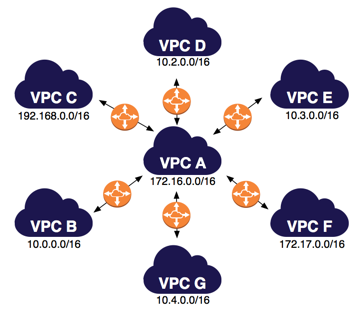
\includegraphics[height=0.8\paperheight]{images/one-to-many-vpcs-diagram.png}
    \end{center}
\end{frame}

% - Once you have functions, types the real fun can begin
% - List comprehensions make these things really easy
% - The AWS API becomes almost legos
\begin{frame}[fragile]{}
    \begin{lstlisting}
    routes: List.concat(
      [
        EC2.Route.new {
          destinationCidrBlock: s.cidrBlock,
          target: EC2.vpcPeeringTarget(s.peerConn),
        } for s in spokeInfos
      ],
      [
        EC2.Route.new {
          destinationCidrBlock: "0.0.0.0/0",
          target: EC2.gatewayTarget(hubNet.igw),
        }
      ]
    )
    \end{lstlisting}
\end{frame}

% - This is a meshed network
% - More expensive to maintain
% - Sometimes needed but yeah it really depends on your application
\begin{frame}{}
    \begin{center}
    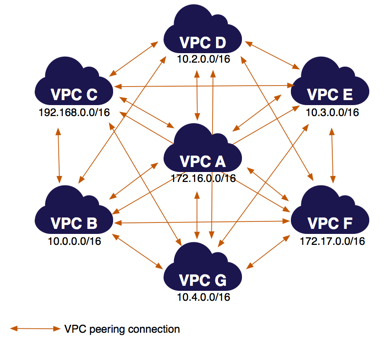
\includegraphics[height=0.8\paperheight]{images/many-vpcs-peered-diagram.png}
    \end{center}
\end{frame}

% - There are clearly people who enjoy a deep satisfaction from writing down route
%   tables like this but I'd rather use a cartesian product
%
% - Keep in mind that this is not everything, all of these will have subnets and
%   gateways and other things which need to be configured
%
% - I used to work in other areas but in my short career in cloud I've seen two
%   people mess this up and spend time debugging it with ping and traceroute and
%   the like.
\begin{frame}[fragile]{}
    \begin{lstlisting}
    VPCs        VPC Peering Connection
    A and B     pcx-aaaabbbb
    A and C     pcx-aaaacccc
    A and D     pcx-aaaadddd
    A and E     pcx-aaaaeeee
    A and F     pcx-aaaaffff
    A and G     pcx-aaaagggg
    B and C     pcx-bbbbcccc
    B and D     pcx-bbbbdddd
    B and E     pcx-bbbbeeee
    B and F     pcx-bbbbffff
    B and G     pcx-bbbbgggg
    C and D     pcx-ccccdddd
    C and E     pcx-cccceeee
    C and F     pcx-ccccffff
    C and G     pcx-ccccgggg
    D and E     pcx-ddddeeee
    D and F     pcx-ddddffff
    D and G     pcx-ddddgggg
    E and F     pcx-eeeeffff
    E and G     pcx-eeeegggg
    F and G     pcx-ffffgggg
    \end{lstlisting}
\end{frame}

% We need to go on about how Infrastructure-as-Code is obviously great idea that
% gives a number of standard benefits such as source control, reproducibility,
% but in the end the ability to experiment really depends on the power of your
% programming language.
%
% You want first-class representations of everything and so on, and once you
% have that...
\blackslide{Infrastructure-as-Code}

\blackslide{Policy-as-Code}

% - You almost get this for free
% - Not really because you need to also build some system for admins to upload
%   and register these
\begin{frame}[fragile]{Policy-as-Code}
    \begin{lstlisting}
    type Result:
      | Ok
      | Error String

    type Rule<a>: fun(a) -> Result
    \end{lstlisting}
\end{frame}

\chapterslide{Questions?}

\end{document}
